\documentclass[mathserif]{beamer}
\usepackage{natbib}
\usepackage{bibentry}
\begin{document}
\nobibliography*
\title{Comparing Adaptive Filtering Techniques \\ ENCE689E --- Reading Assignment}
\author{David Prentiss \\ University of Maryland College Park}
\subtitle{With a summary of \\ \bibentry{crow2008comparison}}

\frame{\titlepage}

\begin{frame}
  \frametitle{Crow and Reichle (2008)}
  \tableofcontents
\end{frame}

\section{Land Surface Modeling}

\begin{frame}
  \frametitle{Crow and Reichle (2008)}
  \tableofcontents[currentsection]
\end{frame}

\begin{frame}
  \frametitle{\insertsection}
  \begin{itemize}
    \item Water and Energy Balance Surface Vegetation Atmosphere Transfer (WEB--SVAT)
    \item Point-based, two-state, mass balance (by volume)
    \item Surface zone (5 cm) moisture flux, $\theta_{sz}$
      \begin{equation}
        \frac{d\theta_{sz}}{dt}=\frac{B_1}{d_{sz}}\left(P_g - E_S\right)-\frac{B_2}{\tau}\left(\theta_{sz}-\theta_{eq}\right)
      \end{equation}
  \end{itemize}
\end{frame}

\begin{frame}
\begin{center}
  \frametitle{\insertsection}
  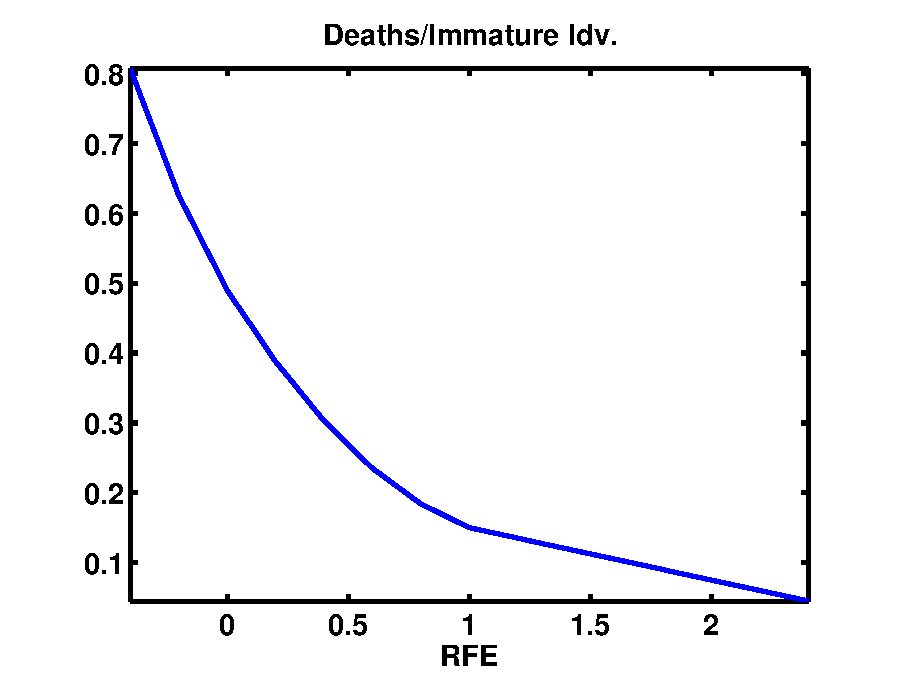
\includegraphics[width=0.9\textwidth]{mortMat}
\end{center}
\end{frame}

\section{EnKFs and Adaptive Filters}

\bibliographystyle{plainnat}
\bibliography{project}
\end{document}
